% Условная компиляция для самостоятельной работы
\ifdefined\mainfile
    % Если это часть основного файла, не добавляем начало и конец документа
\else
    \documentclass[12pt, a4paper]{report}
    \usepackage{/Users/vladbelousov/Desktop/Semestr_4-FP-NSU/Настройка/library}
    \usepackage[utf8]{inputenc} % Подключение поддержки UTF-8
    \begin{document}
\fi

%%-------------------------------%%

1. Интеграл Кирхгофа (поле дифрагированной волны) легко рассчитать на оси круглого отверстия. Вне оси это можно сделать  разложением \( e^{ i kR }  \) по функциям Бесселя, либо разбиением поверхности вторичных источников на зоны Френеля (местами части колец) и интегрированием по азимутальному углу. 

В итоге из-за аксиальной симметрии задачи вне оси наблюдается несколько светлых и темных колец (число \( \approx \) число зон Френеля в отверстии).

2. Принцип Бабине работает для произвольных отверстий и дополняющих эрканов (так как в основе лежит интеграл, то вклад подобластей аддитивен). 

\[ S_2 = S_1 \oplus S_2 \Rightarrow E_{ p_3} = E_{ p_1 } + E_{ p_2 }    \] 

Пример: 

\begin{center}
    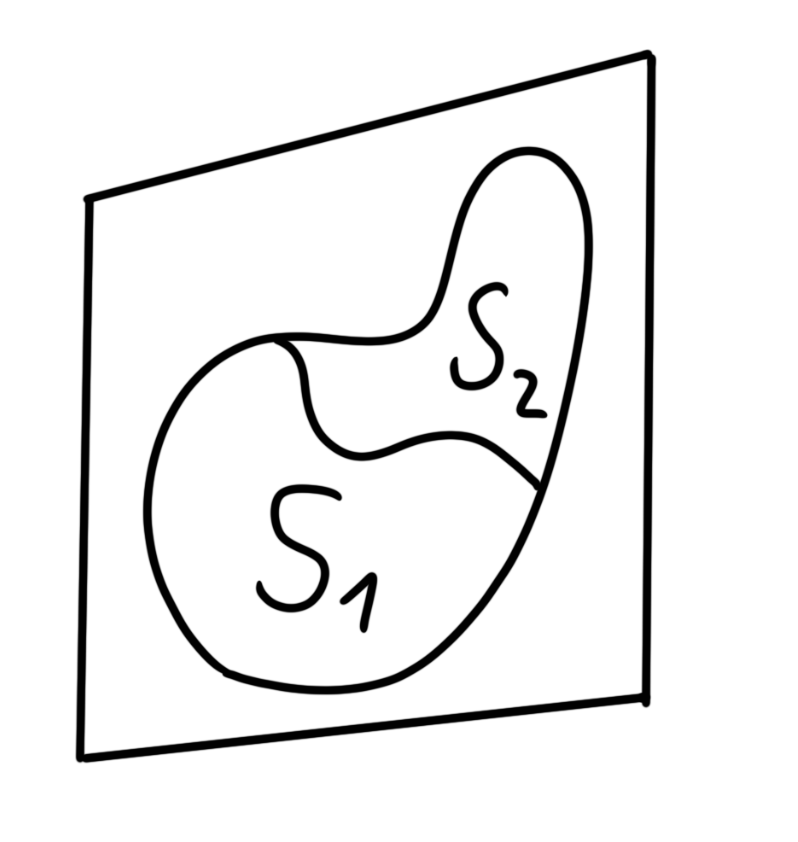
\includegraphics[width=0.3\textwidth]{/Users/vladbelousov/Desktop/Semestr_4-FP-NSU/ЭиО/Лекции_по_дням/image/153.png}
\end{center}

\[ E_p = E_{ p_0} - E_{ p_0} (1 - e^{ i k (R_0 -r )} )   \] 

\begin{center}
    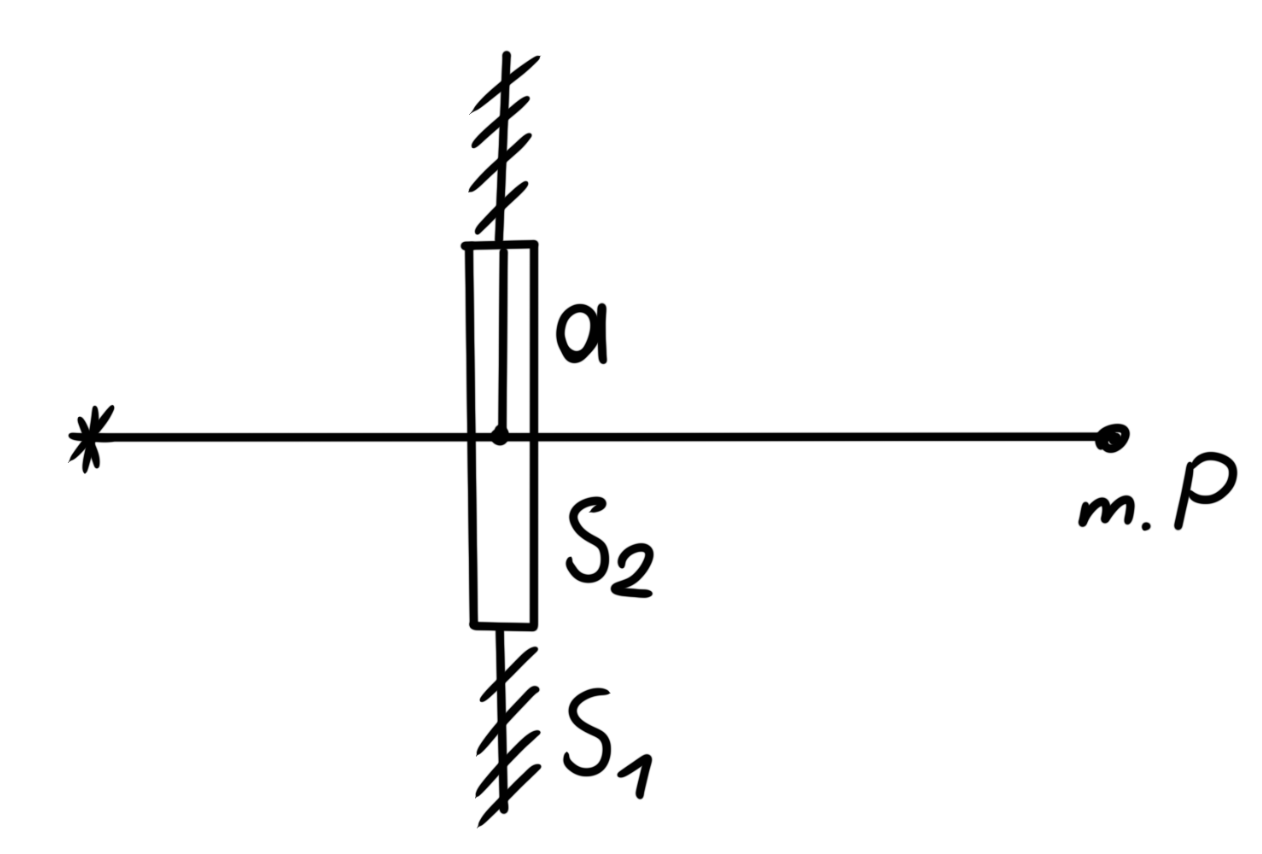
\includegraphics[width=0.5\textwidth]{/Users/vladbelousov/Desktop/Semestr_4-FP-NSU/ЭиО/Лекции_по_дням/image/134.png}
\end{center}

Классификация различных видов дифракции: 

\begin{center}
    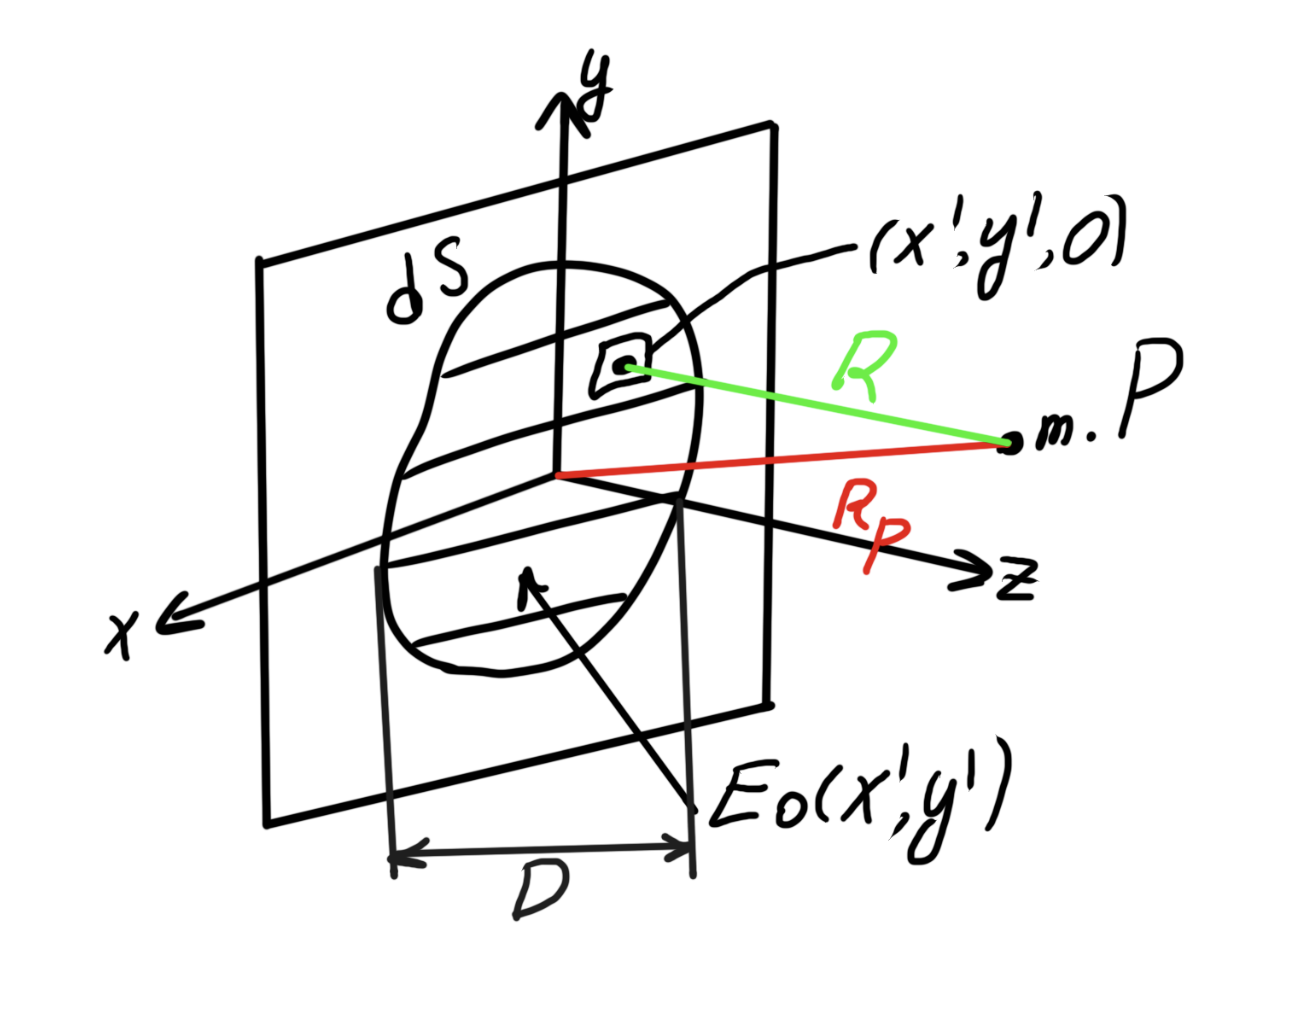
\includegraphics[width=0.5\textwidth]{/Users/vladbelousov/Desktop/Semestr_4-FP-NSU/ЭиО/Лекции_по_дням/image/154.png}
\end{center}
\( dS = dx ' dy ' , \text{ }  R_p = x  ^2 + y ^2 + z ^2   \) 

\[ E_p (x,y ,z ) = \frac{k}{2 \pi i } \iint E_0 (x ', y ' )\frac{ e^{ i k R } }{R } d S_n    \] 

Предположения волны падают на отверстие с небольшими углами и точка \( P \) лежит недалеко от оси. 

\[ R = \sqrt{(x - x' ) ^2 + (y - y ' ) ^2 + z ^2 } = \sqrt{x ^2 + y ^2 + z ^2 - 2 x x' - 2 y y' + (x ' )  ^2  + (y')  ^2  } =[R_p \gg x', y '] \approx  \] 
\[ \approx R_p \left(  1 - \frac{ x x ' }{R_p ^2 } - \frac{y y ' }{R_p ^2 } + \frac{(x' ) ^2 }{2R_p ^2 }+ \frac{ (y ' ) ^2 }{R_p ^2 } + ...       \right) \] 

1 случай: \( \displaystyle  k \frac{ ( x ' ) ^2 }{R_p ^2 } \ll \pi \Rightarrow \frac{ D ^2 }{ \lambda R_p } \ll 1 \quad  \frac{ D ^2 }{\lambda R_p } = P_{\text{Ф} } \text{ - параметр Френеля}      \) 

\[ \Rightarrow P_{\text{Ф} }  \ll 1 \quad  (a_m = \sqrt{m \lambda r } \approx \sqrt{m \lambda }R_p)   \] 

Из \( P_{\text{Ф} } \ll 1 \Rightarrow D \ll a_1 = \sqrt{\lambda}R_p  \) - дифракция Фраунгофера (ссамый простой вид дифракции)

2 случай: \( P_{\text{Ф} } \sim 1  \) - сложная картина дифракции - дифракция Френеля. 

3 случай: \( P_{\text{Ф} } \gg 1   \) = геометрическая оптика 

\begin{center}
    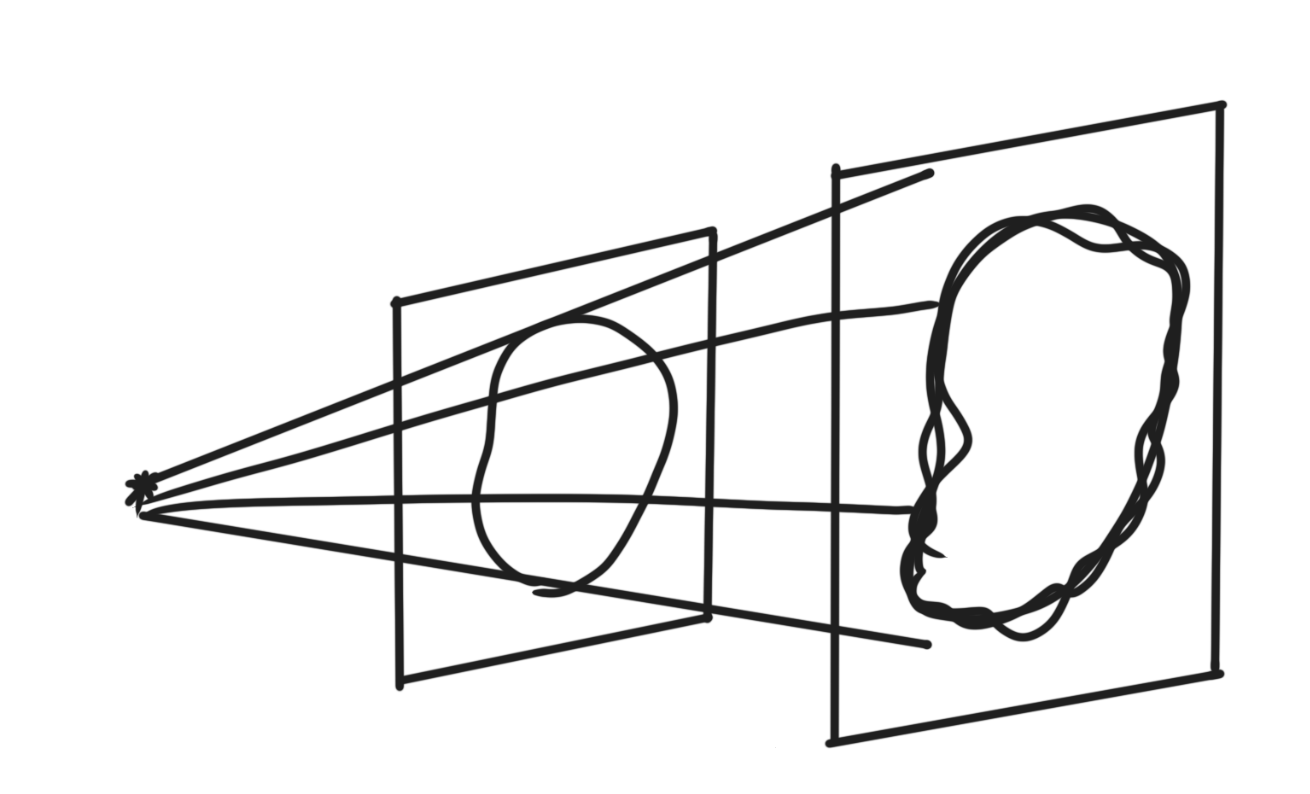
\includegraphics[width=0.5\textwidth]{/Users/vladbelousov/Desktop/Semestr_4-FP-NSU/ЭиО/Лекции_по_дням/image/155.png}
\end{center}
Справа это изображение отверстия 

Вблизи изображения отверстия будут видны дифракционные полосы. \\

Дифракция волны на границе \( \infty  \) плоского экрана: 

\begin{center}
    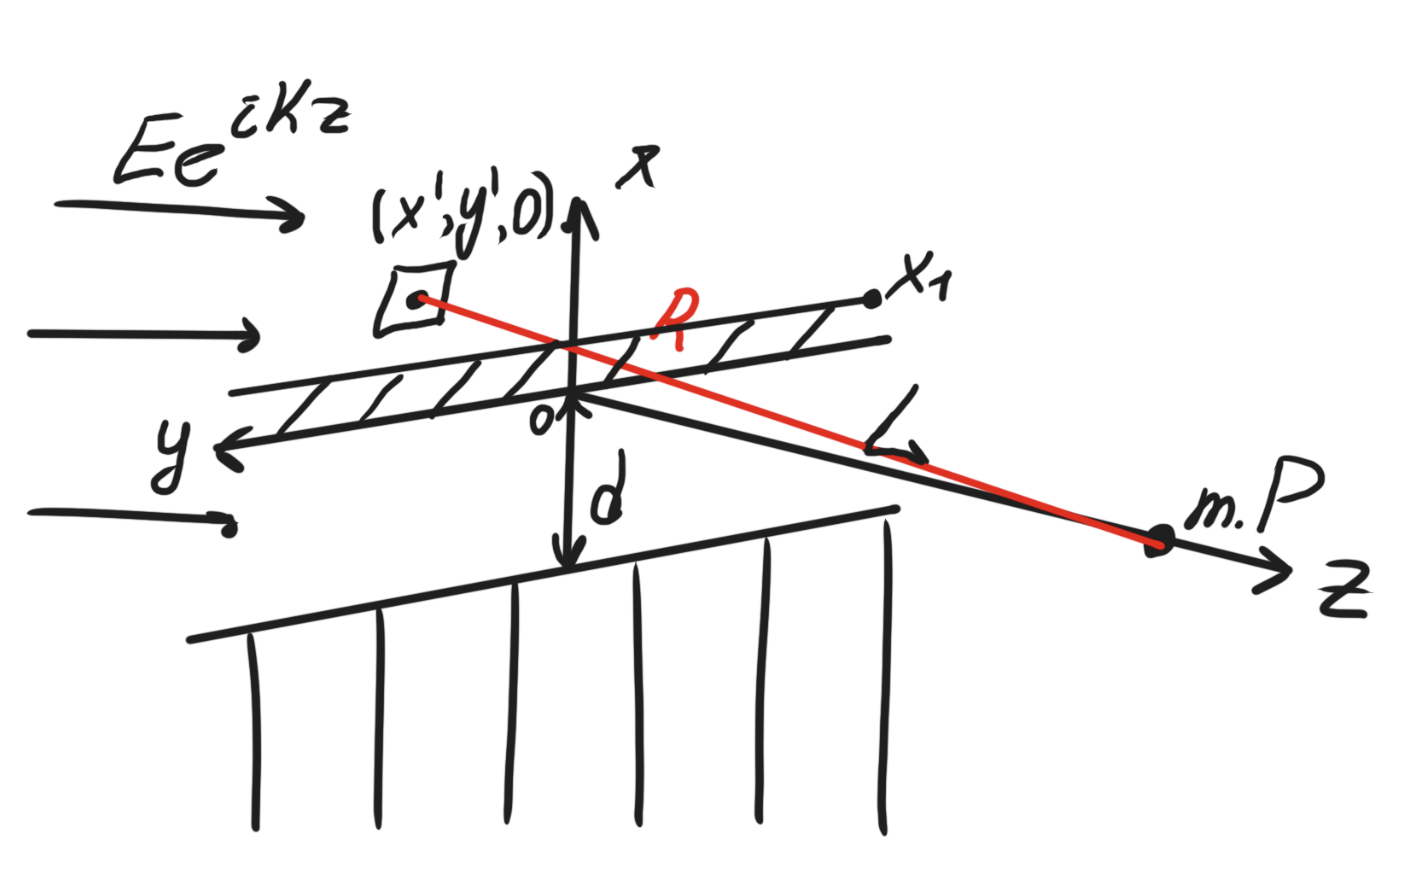
\includegraphics[width=0.5\textwidth]{/Users/vladbelousov/Desktop/Semestr_4-FP-NSU/ЭиО/Лекции_по_дням/image/156.png}
\end{center}

\[ E_p = \frac{k}{ 2 \pi i } \iint  d x ' d y ' \frac{e^{ i kR } }{R } E_0 \] 

\[R = \sqrt{( x ') ^2 + (y ' ) ^2 + L ^2 } \approx L \left( 1 + \frac{ (x ' ) ^2 }{2 L ^2 } + \frac{ (y ' ) ^2 }{2 L ^2 } + ...   \right)  \approx L + \frac{( x ' ) ^2 }{2 L } + \frac{ (y ' ) ^2 }{2 L }   \] 

\[ E_p = \frac{k }{2 \pi i } \frac{E_0 }{L } e^{ik L } \int_{-\infty}^{\infty} e^{ ik \frac{( y ' ) ^2 }{2 L } } d y ' \int_{-d }^{\infty}  e^{ik \frac{( x' ) ^2 }{2L } } dx ' = \frac{k E_0 e^{ i k L } }{2 \pi i L } \sqrt{\frac{\pi 2L }{- i k } } \int_{-d }^{\infty}  e^{ i k \frac{(x ' ) ^2 }{2 L } } dx '     \] 
\[ E_p = E_0 e^{ i k L } \sqrt{\frac{k}{ 2 \pi i L }  } \int_{-d }^{\infty} e^{ i k \frac{(x ' ) ^2 }{2 L } } dx '  \] 

\[\kern-1cm \int_{0 }^{x_1 } e^{ i k \frac{(x ' ) ^2 }{2 L } } dx '  = \left[ \eta  = x' \sqrt{\frac{2}{\lambda L}  } \right] = \sqrt{\frac{\lambda L }{2} }\int_{0 }^{\eta_1} e^{ i \frac{\pi}{2 }  \eta ^2 } d \eta  = \sqrt{\frac{\lambda L }{2} } \bigg(\underbrace{  \int_{ 0 }^{\eta_1 } \cos \left( \frac{\pi \eta ^2 }{2 }  \right) d \eta}_{X(\eta_1 )} + \underbrace{i \int_{0}^{\eta_1 } \sin \left( \frac{\pi \eta ^2 }{2 }  \right) d \eta  }_{Y(\eta_1)} \bigg)   \] 

\begin{center}
    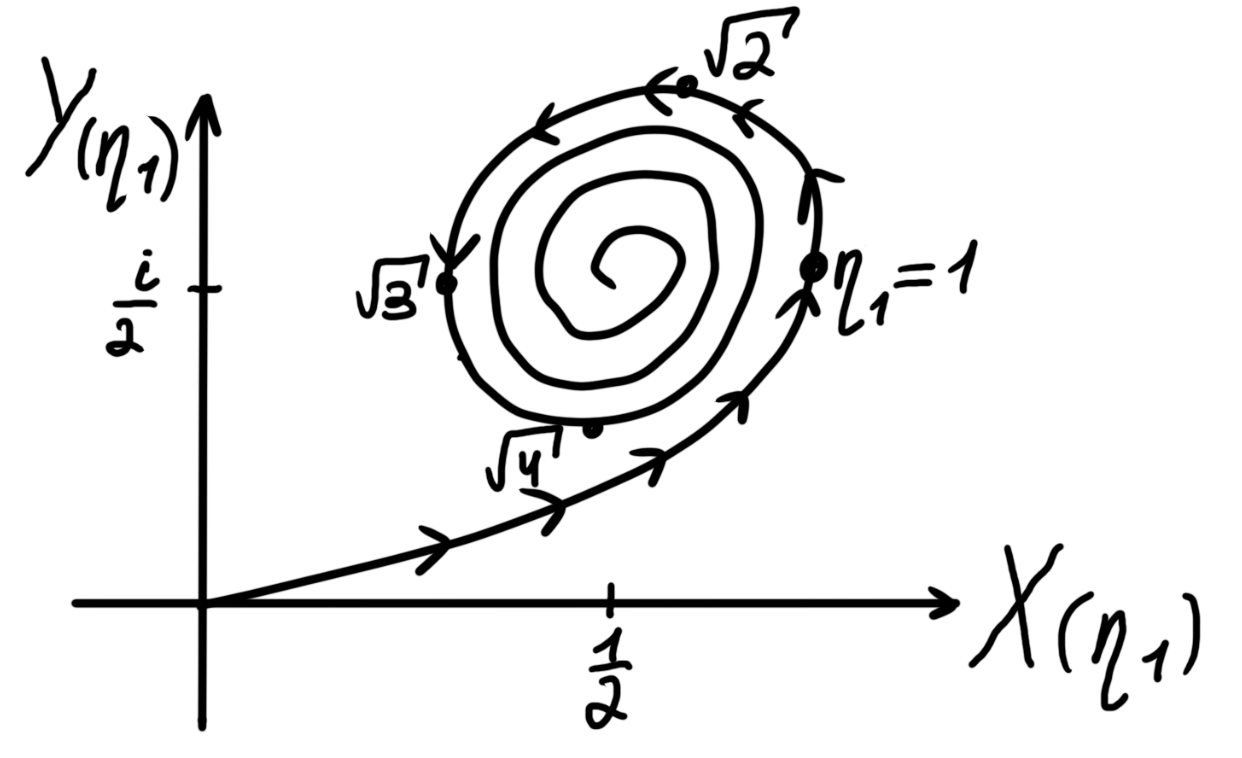
\includegraphics[width=0.5\textwidth]{/Users/vladbelousov/Desktop/Semestr_4-FP-NSU/ЭиО/Лекции_по_дням/image/158.png}
\end{center}


\[ \int_{0}^{\infty} e^{ i \frac{\pi }{2 }\eta  ^2  }d \eta ^2 = \frac{\sqrt[2]{2 i }}{2 } = \frac{ i  +1 }{2 }    \] 
\[ \int_{-|x_1| }^{0 } e^{ ik \frac{ (x ' ) ^2 }{2 L } } d x ' = \sqrt{\frac{ \lambda L }{2 } } \int_{\eta_1 < 0}^{0} e^{ i \frac{\pi}{2 }  \eta ^2 } d \eta = \sqrt{\frac{ \lambda L }{2 } } \int_{0}^{|\eta_1|} e^{ i \frac{\pi}{2 } \eta ^2 }  d \eta      \] 

Тогда графически это влечет следующие изменения:

\begin{center}
    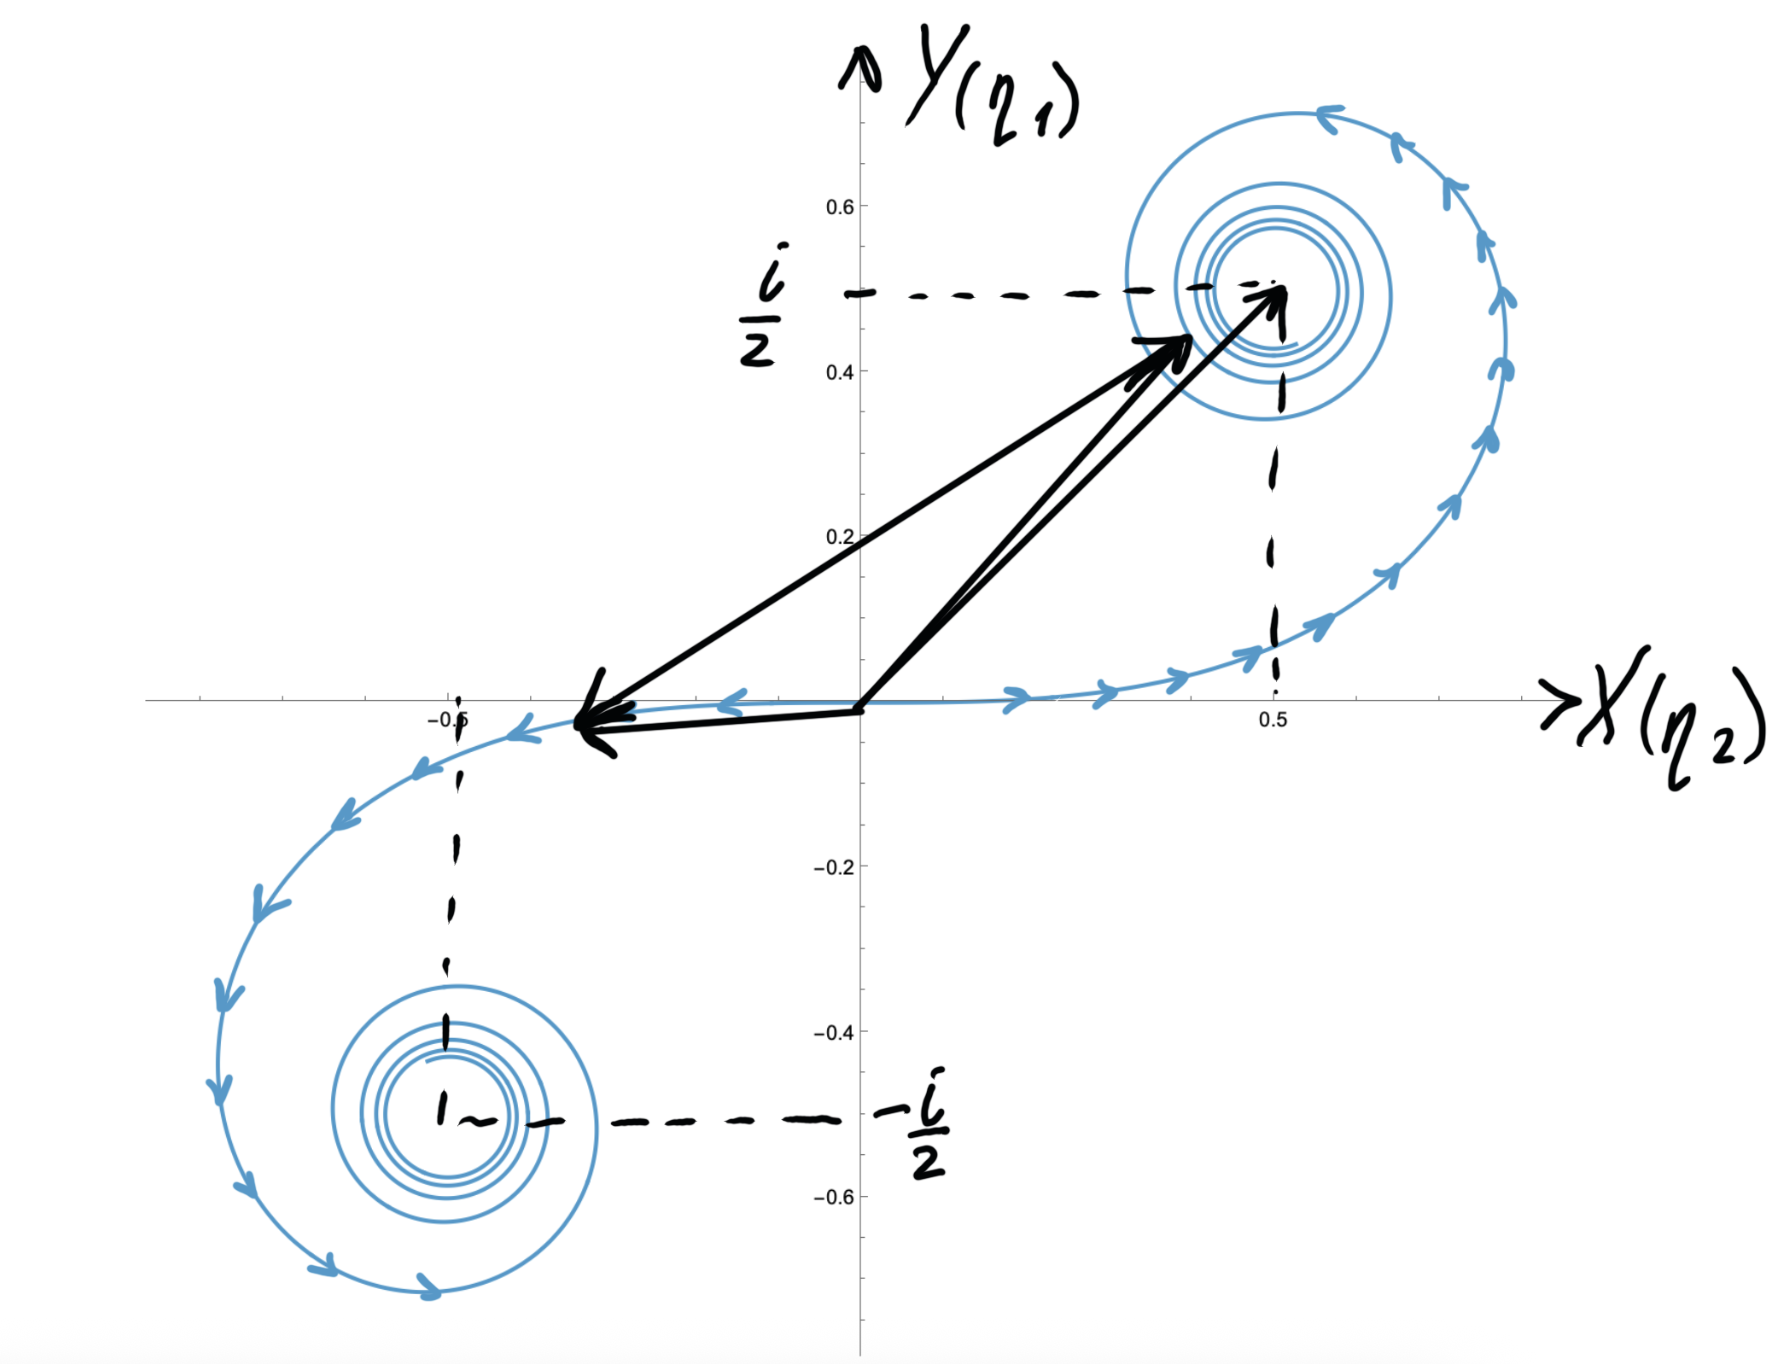
\includegraphics[width=0.5\textwidth]{/Users/vladbelousov/Desktop/Semestr_4-FP-NSU/ЭиО/Лекции_по_дням/image/159.png}
\end{center}
Спираль Корню. \\

1. \( d > 0 \), точка P находится над экраном

\begin{center}
    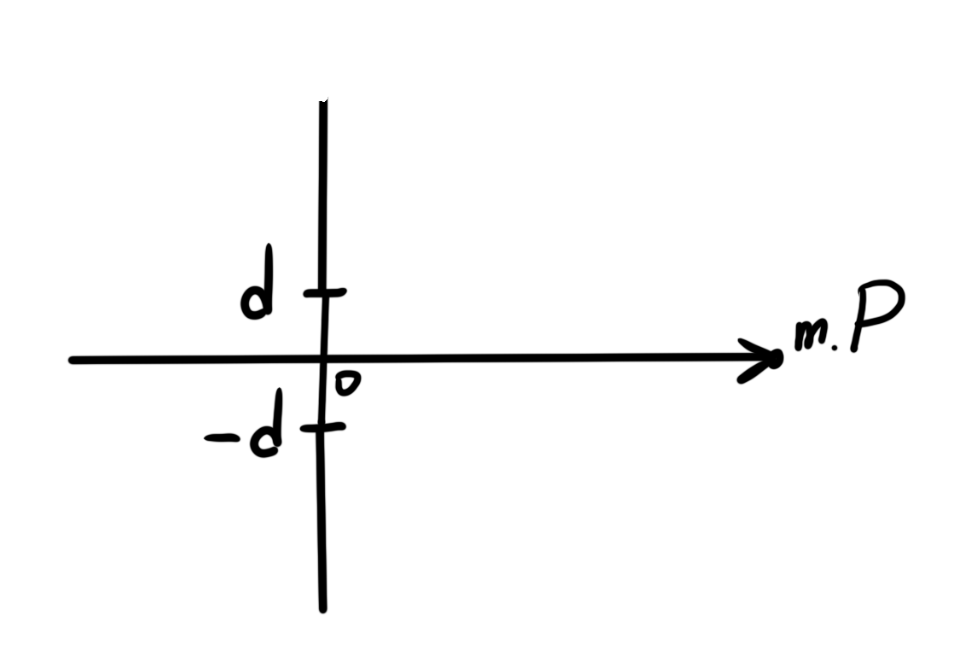
\includegraphics[width=0.3\textwidth]{/Users/vladbelousov/Desktop/Semestr_4-FP-NSU/ЭиО/Лекции_по_дням/image/160.png}
\end{center}


\[ d \gg \frac{ \sqrt{\lambda L }}{2} \quad   \] 
\[ E_p = E_0 e^{i kL } \sqrt{\frac{1}{ i \lambda L } } \bigg( \underbrace{\int_{0}^{\infty}}_{\frac{1}{2} (1 +i)}  + \underbrace{\int_{-\infty}^{0} }_{\frac{1}{2 } (1+ i)} \bigg) \frac{\sqrt{\lambda L }}{2} = E_0 e^{ i kL}  \] 

\begin{center}
    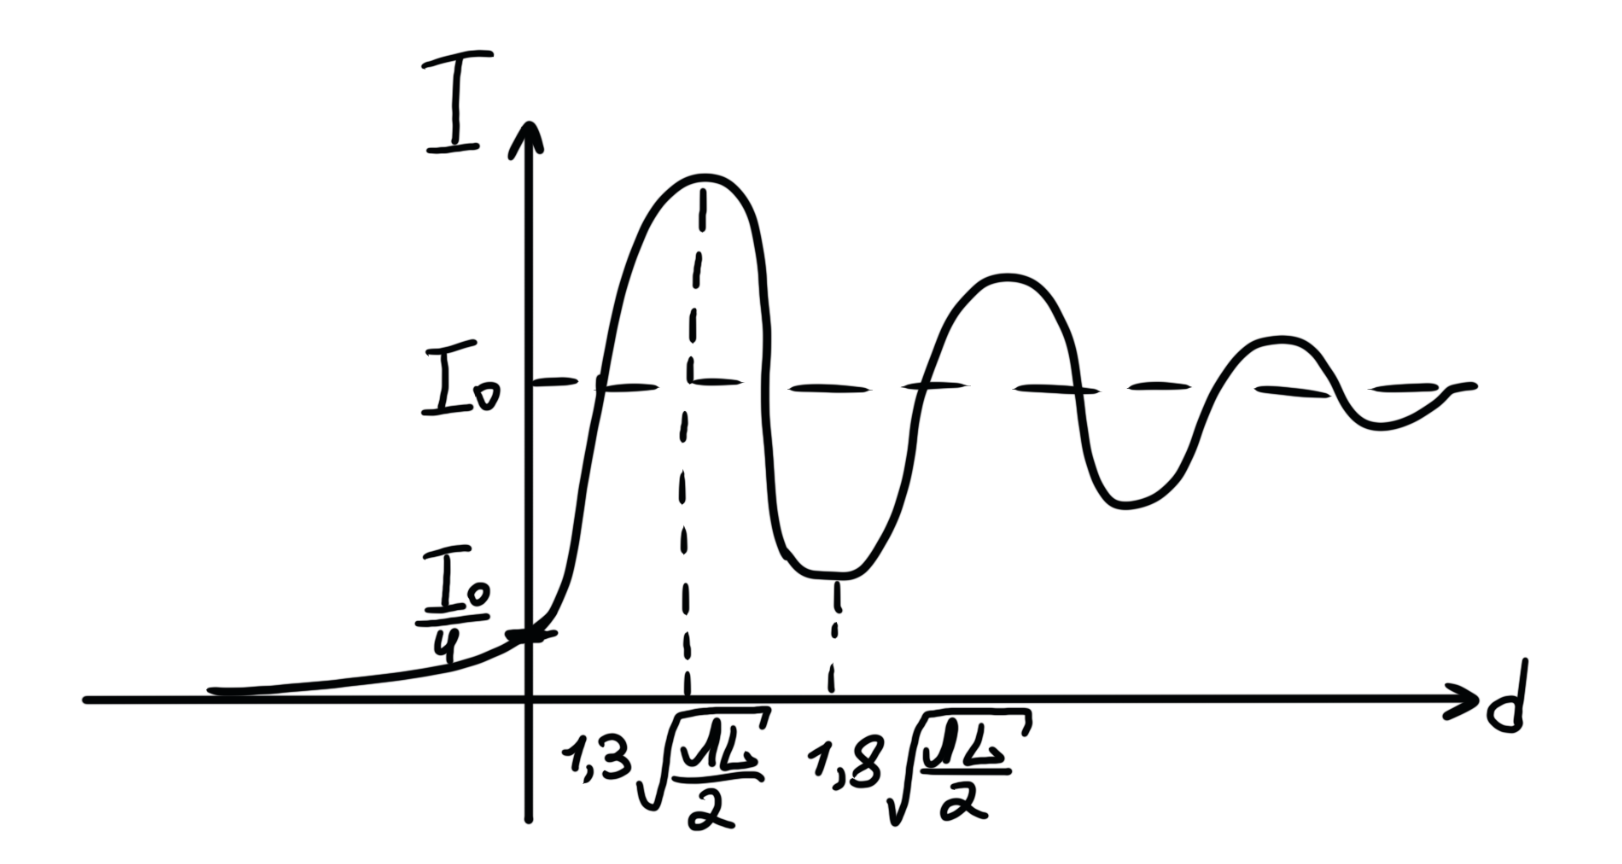
\includegraphics[width=0.6\textwidth]{/Users/vladbelousov/Desktop/Semestr_4-FP-NSU/ЭиО/Лекции_по_дням/image/161.png}
\end{center} 

\[ I_0 = \frac{\left\lvert E_p   \right\rvert ^2 } {2 } = \frac{ \left\lvert E_0 e^{i k L}  \right\rvert ^2 }{2 } = \frac{\left\lvert E_0  \right\rvert ^2 }{2 } = I_0    \] 

Дифракция Фраунгофера: \( \displaystyle  P_{\text{Ф} } = \frac{D ^2 }{\lambda R_{p }  } \ll 1 \Rightarrow \Delta r \ll \lambda    \) 

\[ R \approx R_p \left( 1 - \frac{ x x ' }{R_p ^2 } - \frac{ y y' }{R_p ^2 }   \right) = R_p - \frac{\lambda}{R_p }x '  - \frac{y }{R_p }y '   \] 

\[ E_p = \frac{k}{2 \pi i R_p } \iint dx ' d y ' E(x' , y')   \exp \left( ik \left[ R_p - \frac{x}{R_p }x ' - \frac{y}{R_p }y '   \right]  \right) \cos \theta_0  = \left[ k_x = k \frac{x}{R_p }, \text{ }  k_y = k \frac{y }{R_p }   \right] = \]  
\[ = \frac{k e^{ ik R_p} }{i R_p } \frac{1}{2 \pi } \iint dx ' d y ' E(x' , y' )e^{ - i k_x x '- i k_y y ' } \cos \theta_0 = \frac{k e^{ ik R_p } }{i R_p } \hat{E } (k_x , k_y ) \cos \theta_0       \] 

Случай длинных по \( y \)  щелей \( \Rightarrow  \) удобно использовать интеграл Кирхгофа с цилиндрическими волнами: 

\begin{center}
    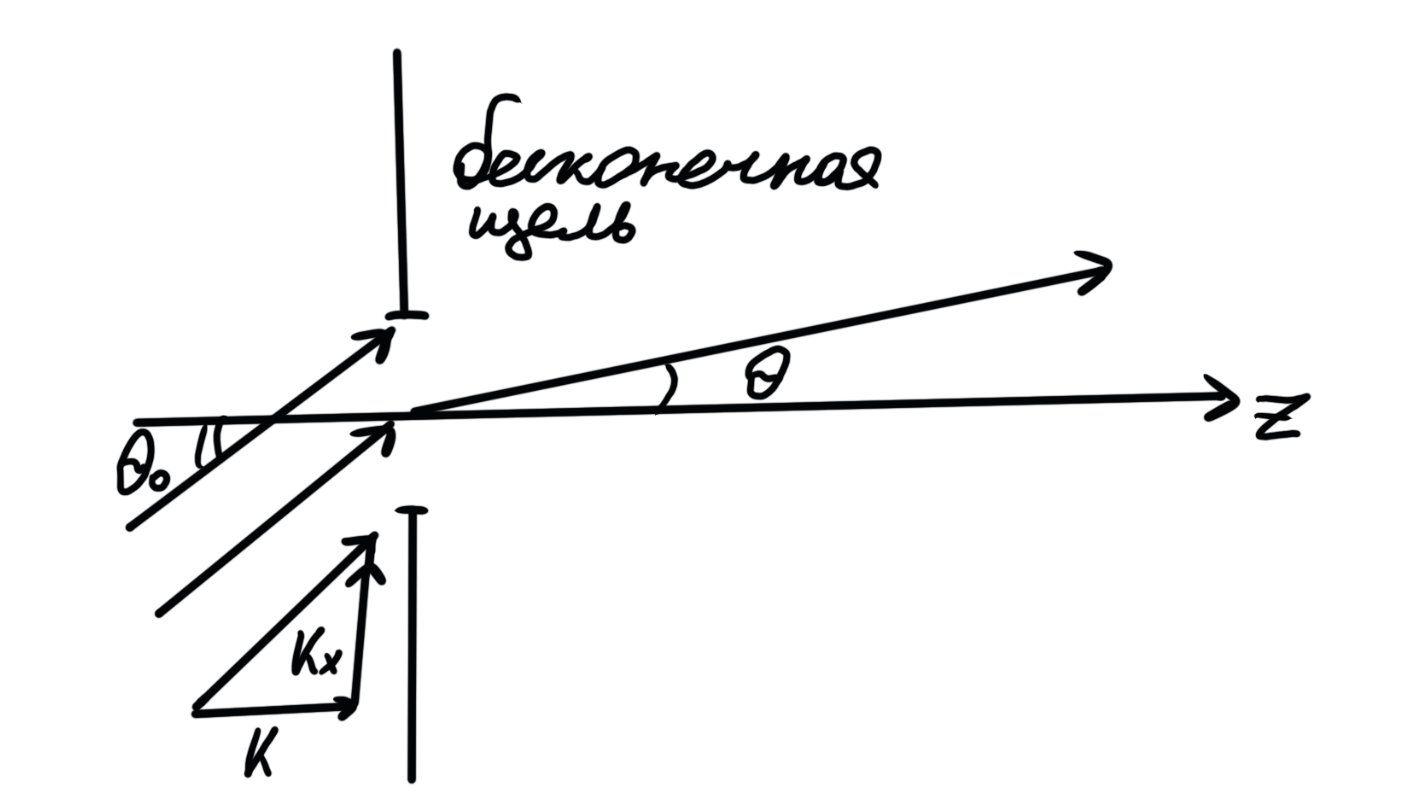
\includegraphics[width=0.5\textwidth]{/Users/vladbelousov/Desktop/Semestr_4-FP-NSU/ЭиО/Лекции_по_дням/image/162.png}
\end{center}

\[ E_p = \sqrt{\frac{k}{ 2 \pi i } } \int_{-\frac{d}{2 } }^{\frac{d}{2} } E(x' ) \frac{e^{i k R} }{\sqrt{R}} dx ' \cos \theta_0   \] 

Распишем компоненты: 

\[ E(x' ) = E_0 e^{i k_0 \sin \theta_0 x '} \quad  k_{0x} = k \sin \theta_0= k \frac{x}{R_p} \quad  e^{i R k} = e^{ ik R_p - i k_x x }     \]  

Итог: 

\[ E_p = \sqrt{\frac{k}{2 \pi i R_p }  } \int_{-\frac{d}{2 } }^{\frac{d}{2} } E_0 e^{ i k_0  \sin  \theta_0 x ' - i k \sin  \theta x' }d x ' e^{ ik R_p }    \cos \theta_0    \] 

%%-------------------------------%%

% Закрытие документа, если файл компилируется отдельно
\ifdefined\mainfile
    % Если это основной файл, не нужно заканчивать документ
\else
    \end{document}
\fi